\section{Time Based Data Analysis (May - August)}

This section filters data for the seasonal months of May through August and visualizes various climate variables including precipitation, humidity, temperature, wind speed, and their distributions.

\subsection*{Filtering Seasonal Months}

\begin{verbatim}
time_based_filter <- df_climate %>%
   dplyr::filter(Month_Label %in% c("May","Jun","Jul","Aug"))
dim(time_based_filter)
\end{verbatim}

\subsection*{Comparison of Precipitation and Humidity by Month}

\begin{verbatim}
precip_temp_data_long <- pivot_longer(precip_temp_data, 
cols = c(Avg_Precip, Avg_humid), 
names_to = "Variable", values_to = "Value")

ggplot(precip_temp_data_long, aes(x = Month_Label, y = Value, 
fill = Variable)) +
geom_bar(stat = "identity", position = "dodge") +
labs(
  title = "Comparison of Precipitation and Humidity by Month",     
  x = "Month", 
  y = "Value") +
  theme_minimal()
\end{verbatim}

% Figure here--------------------
\begin{figure}[h]
    \centering
    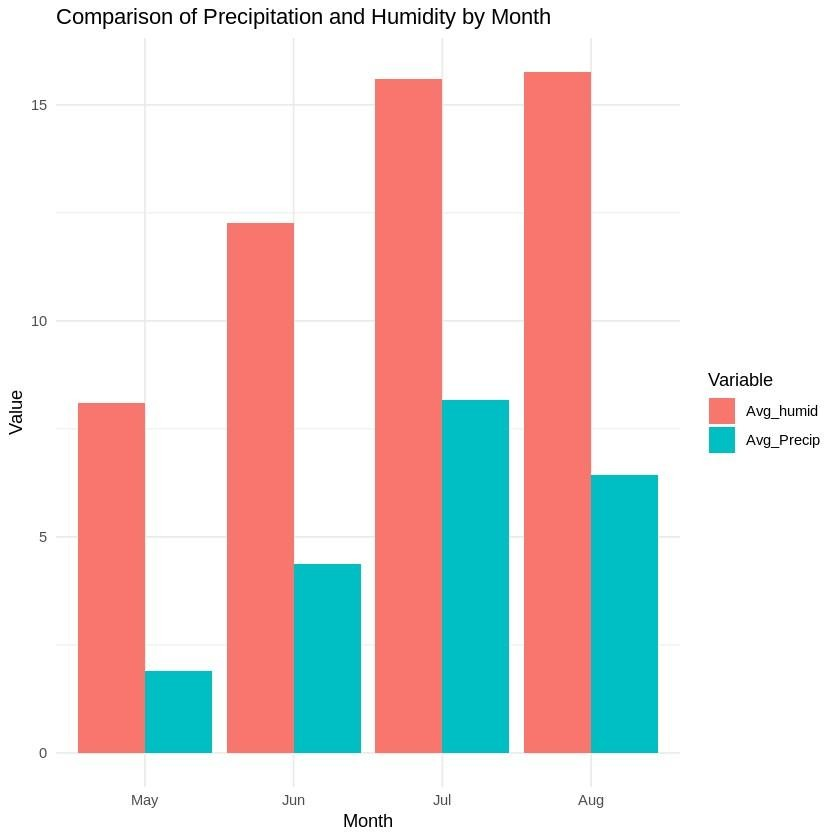
\includegraphics[width=0.5\textwidth]{figures/bar_time.jpg}
    \caption{Bar chart showing precipitation and humidity by month (May to August)}
\end{figure}

\subsection*{Relative Humidity vs Temperature for May to August}

\begin{verbatim}
ggplot(time_based_filter, aes(
  x = Temp_2m, 
  y = RH_2m)) +
geom_point(alpha = 0.3, color = "blue") +
labs(
    title = "Relative Humidity vs Temperature (May - Aug)",
    x = "Temperature (°C)", 
    y = "Relative Humidity (%)") +
  
theme_minimal()
\end{verbatim}

% Figure here-----------------------------
\begin{figure}[h]
    \centering
    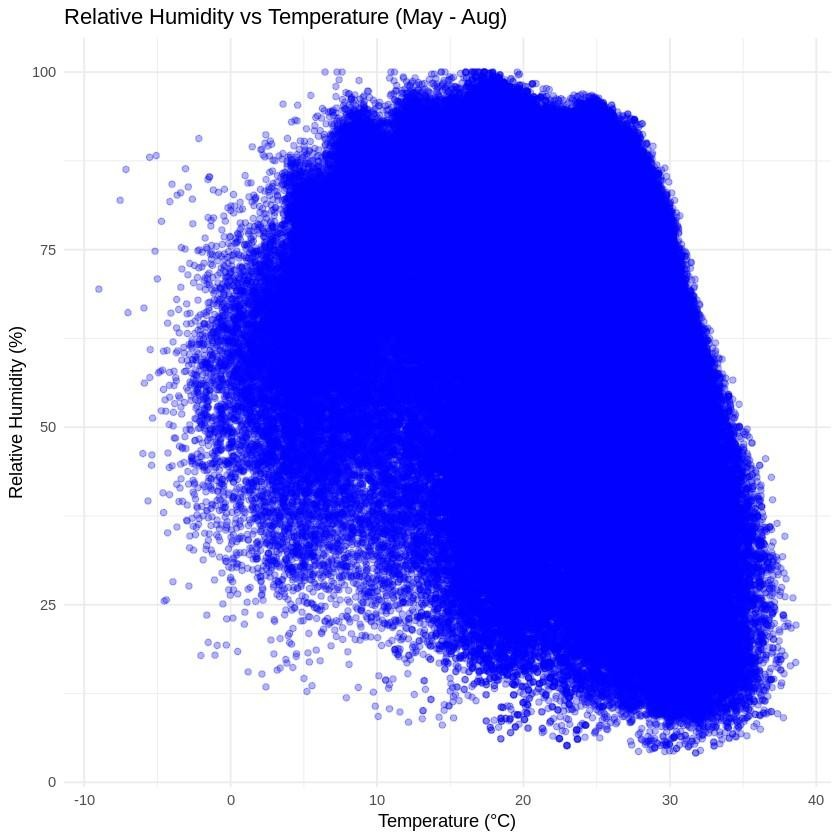
\includegraphics[width=0.5\textwidth]{figures/scatter_time.jpg}
    \caption{Scatterplot showing Temperature vs Relative Humidity (May to August)}
\end{figure}

\subsection*{Wind Speed Range at 10m by Month}

\begin{verbatim}
ggplot(time_based_filter, aes(
  x = Month_Label, 
  y = WindSpeedRange_10m, 
  fill = Month_Label)) +
geom_boxplot() +
labs(
  title = "Wind Speed Range at 10m by Month",
  x = "Month", 
  y = "Wind Speed Range (m/s)") +
  theme_minimal() +
  theme(legend.position = "none")
\end{verbatim}

\begin{figure}[h]
    \centering
    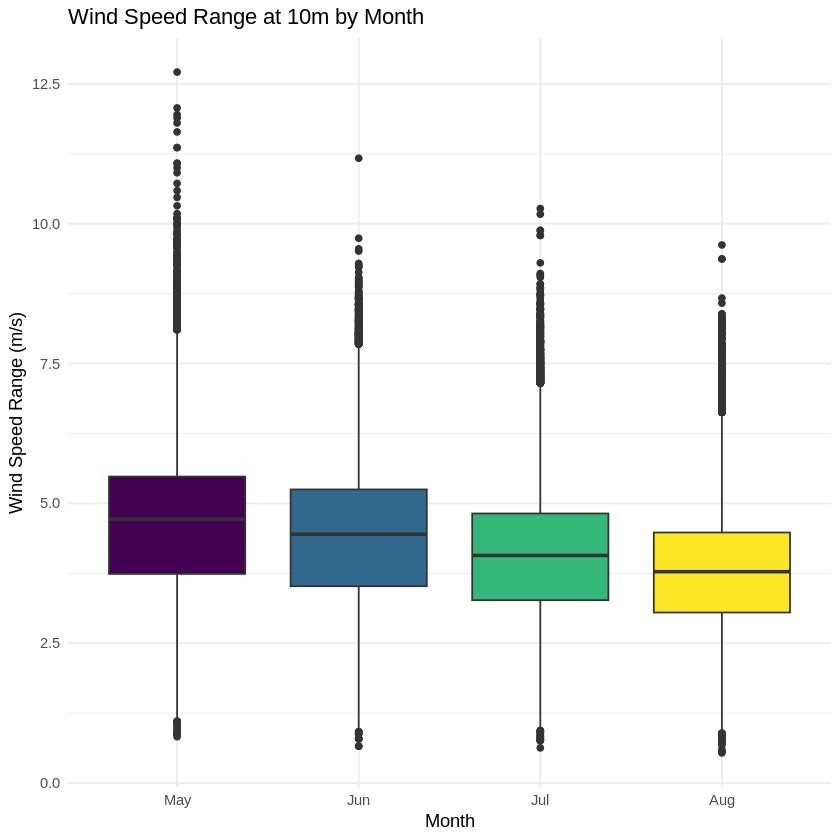
\includegraphics[width=0.5\textwidth]{figures/box_time.jpg}
    \caption{Boxplot of Wind Speed Range at 10m by Month (May to August)}
\end{figure}

\subsection*{Average Temperature Heatmap by District and Month}

To find out how temperature varies by district across different months, we created a heatmap that shows the average temperature for each district by month. This visualization helps us quickly identify seasonal patterns and regional differences in temperature across Nepal.
\begin{verbatim}
library(reshape2)

avg_temp_district <- time_based_filter %>%
  group_by(District, Month_Label) %>%
  summarise(
    AvgTemp = mean(Temp_2m, na.rm = TRUE)) %>%
  ungroup()

ggplot(avg_temp_district, aes(
  x = Month_Label, 
  y = District, 
  fill = AvgTemp)) +
  geom_tile() +
  scale_fill_viridis_c(option = "plasma") +
  labs(
    title = "Average Temperature by District and Month",
    x = "Month", 
    y = "District", 
    fill = "Avg Temp (°C)") +

  theme_minimal() +

  theme(axis.text.y = element_text(size = 6))
\end{verbatim}

% Figure here-----------------------------
\begin{figure}[h]
    \centering
    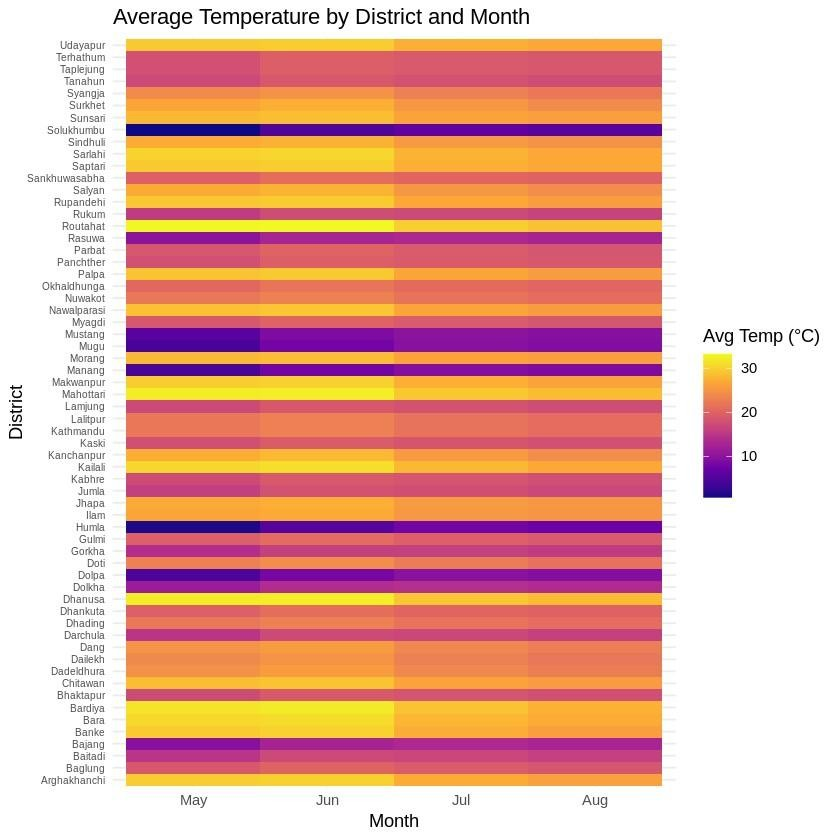
\includegraphics[width=0.6\textwidth]{figures/heatmap_time.jpg}
    \caption{Average Temperature Heatmap by District and Month (May to August)}
    \label{fig:avg_temp_heatmap}
\end{figure}

\subsection*{Density Plot of Temperature by Month}

\begin{verbatim}
ggplot(time_based_filter, aes(x = Temp_2m, fill = Month_Label)) +
  geom_density(alpha = 0.5) +
  labs(title = "Temperature Density by Month (May-August)",
       x = "Temperature (°C)", y = "Density") +
  theme_minimal()
\end{verbatim}

% Figure here------------------------
\begin{figure}[h]
    \centering
    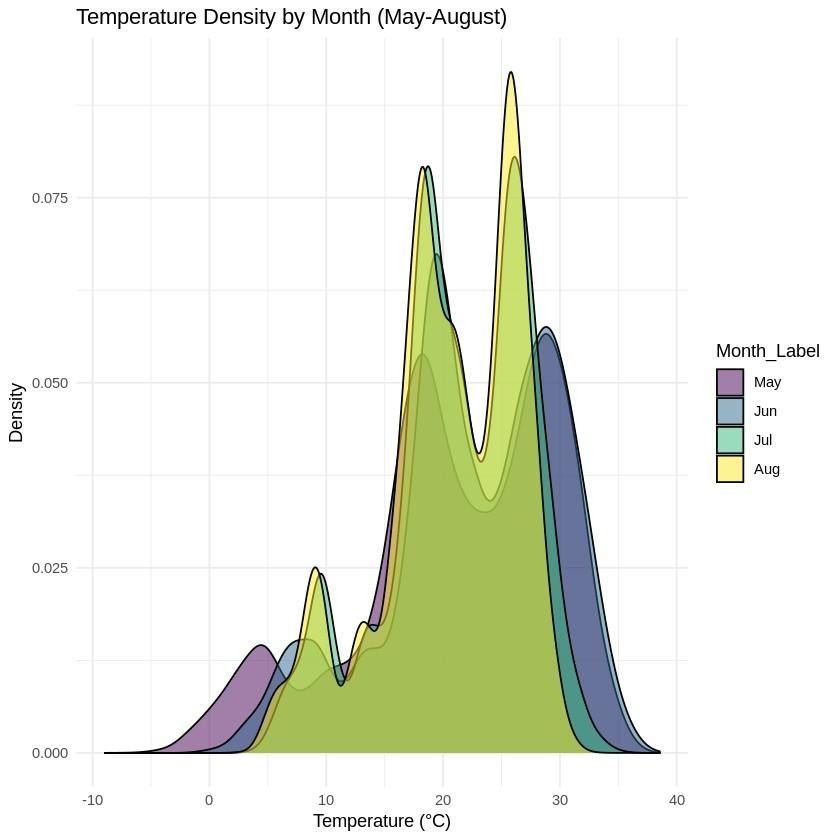
\includegraphics[width=0.45\textwidth]{figures/density_time.jpg}
    \caption{Density plot of Temperature distribution by month (May to August)}
    \label{fig:temp_density}
\end{figure}
